% Options for packages loaded elsewhere
\PassOptionsToPackage{unicode}{hyperref}
\PassOptionsToPackage{hyphens}{url}
%
\documentclass[
]{article}
\usepackage{amsmath,amssymb}
\usepackage{iftex}
\ifPDFTeX
  \usepackage[T1]{fontenc}
  \usepackage[utf8]{inputenc}
  \usepackage{textcomp} % provide euro and other symbols
\else % if luatex or xetex
  \usepackage{unicode-math} % this also loads fontspec
  \defaultfontfeatures{Scale=MatchLowercase}
  \defaultfontfeatures[\rmfamily]{Ligatures=TeX,Scale=1}
\fi
\usepackage{lmodern}
\ifPDFTeX\else
  % xetex/luatex font selection
\fi
% Use upquote if available, for straight quotes in verbatim environments
\IfFileExists{upquote.sty}{\usepackage{upquote}}{}
\IfFileExists{microtype.sty}{% use microtype if available
  \usepackage[]{microtype}
  \UseMicrotypeSet[protrusion]{basicmath} % disable protrusion for tt fonts
}{}
\makeatletter
\@ifundefined{KOMAClassName}{% if non-KOMA class
  \IfFileExists{parskip.sty}{%
    \usepackage{parskip}
  }{% else
    \setlength{\parindent}{0pt}
    \setlength{\parskip}{6pt plus 2pt minus 1pt}}
}{% if KOMA class
  \KOMAoptions{parskip=half}}
\makeatother
\usepackage{xcolor}
\usepackage[a4paper]{geometry}
\usepackage{color}
\usepackage{fancyvrb}
\newcommand{\VerbBar}{|}
\newcommand{\VERB}{\Verb[commandchars=\\\{\}]}
\DefineVerbatimEnvironment{Highlighting}{Verbatim}{commandchars=\\\{\}}
% Add ',fontsize=\small' for more characters per line
\usepackage{framed}
\definecolor{shadecolor}{RGB}{248,248,248}
\newenvironment{Shaded}{\begin{snugshade}}{\end{snugshade}}
\newcommand{\AlertTok}[1]{\textcolor[rgb]{0.94,0.16,0.16}{#1}}
\newcommand{\AnnotationTok}[1]{\textcolor[rgb]{0.56,0.35,0.01}{\textbf{\textit{#1}}}}
\newcommand{\AttributeTok}[1]{\textcolor[rgb]{0.13,0.29,0.53}{#1}}
\newcommand{\BaseNTok}[1]{\textcolor[rgb]{0.00,0.00,0.81}{#1}}
\newcommand{\BuiltInTok}[1]{#1}
\newcommand{\CharTok}[1]{\textcolor[rgb]{0.31,0.60,0.02}{#1}}
\newcommand{\CommentTok}[1]{\textcolor[rgb]{0.56,0.35,0.01}{\textit{#1}}}
\newcommand{\CommentVarTok}[1]{\textcolor[rgb]{0.56,0.35,0.01}{\textbf{\textit{#1}}}}
\newcommand{\ConstantTok}[1]{\textcolor[rgb]{0.56,0.35,0.01}{#1}}
\newcommand{\ControlFlowTok}[1]{\textcolor[rgb]{0.13,0.29,0.53}{\textbf{#1}}}
\newcommand{\DataTypeTok}[1]{\textcolor[rgb]{0.13,0.29,0.53}{#1}}
\newcommand{\DecValTok}[1]{\textcolor[rgb]{0.00,0.00,0.81}{#1}}
\newcommand{\DocumentationTok}[1]{\textcolor[rgb]{0.56,0.35,0.01}{\textbf{\textit{#1}}}}
\newcommand{\ErrorTok}[1]{\textcolor[rgb]{0.64,0.00,0.00}{\textbf{#1}}}
\newcommand{\ExtensionTok}[1]{#1}
\newcommand{\FloatTok}[1]{\textcolor[rgb]{0.00,0.00,0.81}{#1}}
\newcommand{\FunctionTok}[1]{\textcolor[rgb]{0.13,0.29,0.53}{\textbf{#1}}}
\newcommand{\ImportTok}[1]{#1}
\newcommand{\InformationTok}[1]{\textcolor[rgb]{0.56,0.35,0.01}{\textbf{\textit{#1}}}}
\newcommand{\KeywordTok}[1]{\textcolor[rgb]{0.13,0.29,0.53}{\textbf{#1}}}
\newcommand{\NormalTok}[1]{#1}
\newcommand{\OperatorTok}[1]{\textcolor[rgb]{0.81,0.36,0.00}{\textbf{#1}}}
\newcommand{\OtherTok}[1]{\textcolor[rgb]{0.56,0.35,0.01}{#1}}
\newcommand{\PreprocessorTok}[1]{\textcolor[rgb]{0.56,0.35,0.01}{\textit{#1}}}
\newcommand{\RegionMarkerTok}[1]{#1}
\newcommand{\SpecialCharTok}[1]{\textcolor[rgb]{0.81,0.36,0.00}{\textbf{#1}}}
\newcommand{\SpecialStringTok}[1]{\textcolor[rgb]{0.31,0.60,0.02}{#1}}
\newcommand{\StringTok}[1]{\textcolor[rgb]{0.31,0.60,0.02}{#1}}
\newcommand{\VariableTok}[1]{\textcolor[rgb]{0.00,0.00,0.00}{#1}}
\newcommand{\VerbatimStringTok}[1]{\textcolor[rgb]{0.31,0.60,0.02}{#1}}
\newcommand{\WarningTok}[1]{\textcolor[rgb]{0.56,0.35,0.01}{\textbf{\textit{#1}}}}
\usepackage{graphicx}
\makeatletter
\def\maxwidth{\ifdim\Gin@nat@width>\linewidth\linewidth\else\Gin@nat@width\fi}
\def\maxheight{\ifdim\Gin@nat@height>\textheight\textheight\else\Gin@nat@height\fi}
\makeatother
% Scale images if necessary, so that they will not overflow the page
% margins by default, and it is still possible to overwrite the defaults
% using explicit options in \includegraphics[width, height, ...]{}
\setkeys{Gin}{width=\maxwidth,height=\maxheight,keepaspectratio}
% Set default figure placement to htbp
\makeatletter
\def\fps@figure{htbp}
\makeatother
\setlength{\emergencystretch}{3em} % prevent overfull lines
\providecommand{\tightlist}{%
  \setlength{\itemsep}{0pt}\setlength{\parskip}{0pt}}
\setcounter{secnumdepth}{5}
\usepackage{booktabs}
\usepackage{longtable}
\usepackage{array}
\usepackage{multirow}
\usepackage{wrapfig}
\usepackage{float}
\usepackage{colortbl}
\usepackage{pdflscape}
\usepackage{tabu}
\usepackage{threeparttable}
\usepackage{threeparttablex}
\usepackage[normalem]{ulem}
\usepackage{makecell}
\usepackage{xcolor}
\usepackage{caption}
\usepackage{anyfontsize}
\ifLuaTeX
  \usepackage{selnolig}  % disable illegal ligatures
\fi
\usepackage{bookmark}
\IfFileExists{xurl.sty}{\usepackage{xurl}}{} % add URL line breaks if available
\urlstyle{same}
\hypersetup{
  pdftitle={Assessment: Predicting Length of Stay for Hospitalised Covid-19 Patients Using Random Forest Machine Learning},
  pdfauthor={B273025},
  hidelinks,
  pdfcreator={LaTeX via pandoc}}

\title{Assessment: Predicting Length of Stay for Hospitalised Covid-19
Patients Using Random Forest Machine Learning}
\author{B273025}
\date{2024-11-16}

\begin{document}
\maketitle

\section{Introduction}\label{introduction}

The Covid-19 Pandemic placed unprecedented strain on health systems,
making resource allocation essential to prevent services from being
overwhelmed. Predicting hospital demand, including bed occupancy,
staffing needs and equipment requirements, became critical for informed
decision-making(1).

Hospital demand depends on two factors:

\begin{enumerate}
\def\labelenumi{\arabic{enumi}.}
\item
  The number of individuals requiring hospitalisation, estimated using
  epidemic curves.
\item
  The length of hospital stay (LOS), derived from patient observations.
\end{enumerate}

This report develops a model to predict LOS for hospitalised Covid-19
patients based on individual factors. Accurate LOS predictions support:

\begin{enumerate}
\def\labelenumi{\arabic{enumi}.}
\item
  Optimised resource allocation
\item
  Improved patient care and logistic planning
\item
  Enhanced pandemic preparedness
\end{enumerate}

\begin{Shaded}
\begin{Highlighting}[]
\CommentTok{\#Load necessary libraries:}
\FunctionTok{library}\NormalTok{(sparklyr)}
\FunctionTok{library}\NormalTok{(dplyr)}
\FunctionTok{library}\NormalTok{(purrr)}
\FunctionTok{library}\NormalTok{(ggplot2)}
\FunctionTok{library}\NormalTok{(broom)}
\FunctionTok{library}\NormalTok{(gt)}
\FunctionTok{library}\NormalTok{(knitr)}
\FunctionTok{library}\NormalTok{(corrr)}
\FunctionTok{library}\NormalTok{(kableExtra)}
\end{Highlighting}
\end{Shaded}

\begin{Shaded}
\begin{Highlighting}[]
\CommentTok{\#Connect to spark and read in data:}
\CommentTok{\# connects to local machine as if it were a cluster }
\NormalTok{sc }\OtherTok{=} \FunctionTok{spark\_connect}\NormalTok{(}\AttributeTok{master =} \StringTok{\textquotesingle{}local\textquotesingle{}}\NormalTok{)}
\CommentTok{\# load the dataset into spark (sdf = spark dataframe) }
\NormalTok{sdf\_covid\_hosp }\OtherTok{\textless{}{-}} \FunctionTok{spark\_read\_csv}\NormalTok{(sc, }\StringTok{\textquotesingle{}host\_train.csv\textquotesingle{}}\NormalTok{)}
\end{Highlighting}
\end{Shaded}

\section{Exploratory Data Analysis}\label{exploratory-data-analysis}

\begin{Shaded}
\begin{Highlighting}[]
\CommentTok{\# Define a function to summarise the spark dataframe (sdf) efficiently}
\CommentTok{\# note this function is applicable in a big data setting where there are a manageable number of columns (as is the case with this dataset)}

\NormalTok{summarise\_big\_data }\OtherTok{\textless{}{-}} \ControlFlowTok{function}\NormalTok{(sdf, }\AttributeTok{cardinality\_limit =} \DecValTok{15}\NormalTok{) \{}
  \CommentTok{\# Retrieve schema to extract column names}
\NormalTok{  schema }\OtherTok{\textless{}{-}} \FunctionTok{sdf\_schema}\NormalTok{(sdf)}
  
  \CommentTok{\# Iterate over schema to compute metrics for each column}
\NormalTok{  metrics }\OtherTok{\textless{}{-}}\NormalTok{ purrr}\SpecialCharTok{::}\FunctionTok{map\_dfr}\NormalTok{(schema, }\SpecialCharTok{\textasciitilde{}}\NormalTok{ \{}
\NormalTok{    col\_name }\OtherTok{\textless{}{-}}\NormalTok{ .x}\SpecialCharTok{$}\NormalTok{name  }\CommentTok{\# Extract column name}
    \CommentTok{\# Compute cardinality and missing percentage in Spark}
\NormalTok{    summary\_spark }\OtherTok{\textless{}{-}}\NormalTok{ sdf }\SpecialCharTok{\%\textgreater{}\%}
      \FunctionTok{summarise}\NormalTok{(}\AttributeTok{cardinality =} \FunctionTok{approx\_count\_distinct}\NormalTok{(}\SpecialCharTok{!!}\FunctionTok{sym}\NormalTok{(col\_name)),  }\CommentTok{\# Approximate distinct count for efficiency}
                \AttributeTok{nans\_pct =}\NormalTok{ (}\FunctionTok{sum}\NormalTok{(}\FunctionTok{ifelse}\NormalTok{(}\FunctionTok{is.na}\NormalTok{(}\SpecialCharTok{!!}\FunctionTok{sym}\NormalTok{(col\_name)), }\DecValTok{1}\NormalTok{, }\DecValTok{0}\NormalTok{)) }\SpecialCharTok{/} \FunctionTok{n}\NormalTok{()) }\SpecialCharTok{*} \DecValTok{100}\NormalTok{) }\SpecialCharTok{\%\textgreater{}\%}   \CommentTok{\# Percent missing}
      \FunctionTok{collect}\NormalTok{()  }\CommentTok{\# Collect results into R}
    
    \CommentTok{\# Extract cardinality and missing percentage from the collected summary}
\NormalTok{    cardinality }\OtherTok{\textless{}{-}}\NormalTok{ summary\_spark }\SpecialCharTok{\%\textgreater{}\%} \FunctionTok{pull}\NormalTok{(cardinality)}
\NormalTok{    nans\_pct }\OtherTok{\textless{}{-}}\NormalTok{ summary\_spark }\SpecialCharTok{\%\textgreater{}\%} \FunctionTok{pull}\NormalTok{(nans\_pct)}
    
    \CommentTok{\# If cardinality is low, extract sample categories in Spark}
\NormalTok{    categories\_str }\OtherTok{\textless{}{-}} \ControlFlowTok{if}\NormalTok{ (cardinality }\SpecialCharTok{\textless{}}\NormalTok{ cardinality\_limit) \{}
\NormalTok{      sdf }\SpecialCharTok{\%\textgreater{}\%}
        \FunctionTok{select}\NormalTok{(}\SpecialCharTok{!!}\FunctionTok{sym}\NormalTok{(col\_name)) }\SpecialCharTok{\%\textgreater{}\%}
        \FunctionTok{distinct}\NormalTok{() }\SpecialCharTok{\%\textgreater{}\%}
        \FunctionTok{head}\NormalTok{(cardinality\_limit) }\SpecialCharTok{\%\textgreater{}\%}
        \FunctionTok{collect}\NormalTok{() }\SpecialCharTok{\%\textgreater{}\%}
        \FunctionTok{pull}\NormalTok{(}\SpecialCharTok{!!}\FunctionTok{sym}\NormalTok{(col\_name)) }\SpecialCharTok{\%\textgreater{}\%}
        \FunctionTok{paste}\NormalTok{(}\AttributeTok{collapse =} \StringTok{", "}\NormalTok{)}
\NormalTok{    \} }\ControlFlowTok{else}\NormalTok{ \{}
      \ConstantTok{NA}\NormalTok{\}  }\CommentTok{\# Skip for high{-}cardinality columns}
  
    \CommentTok{\# Combine results into a data frame row}
    \FunctionTok{tibble}\NormalTok{(}
      \AttributeTok{feature =}\NormalTok{ col\_name,}
      \AttributeTok{cardinality =}\NormalTok{ cardinality,}
      \AttributeTok{nans\_pct =}\NormalTok{ nans\_pct,}
      \AttributeTok{categories =}\NormalTok{ categories\_str)\})}
  \FunctionTok{return}\NormalTok{(metrics)\}}

\CommentTok{\# Apply the function to the Spark DataFrame}
\NormalTok{ldf\_summary\_table }\OtherTok{\textless{}{-}} \FunctionTok{summarise\_big\_data}\NormalTok{(sdf\_covid\_hosp)}

\CommentTok{\# Present summary in a table }
\NormalTok{ldf\_summary\_table }\OtherTok{\textless{}{-}}\NormalTok{ ldf\_summary\_table }\SpecialCharTok{\%\textgreater{}\%} 
  \FunctionTok{select}\NormalTok{(feature, categories, cardinality, nans\_pct) }\SpecialCharTok{\%\textgreater{}\%} \CommentTok{\# order columns for table}
  \FunctionTok{gt}\NormalTok{(}\AttributeTok{rowname\_col =} \StringTok{"feature"}\NormalTok{) }\SpecialCharTok{\%\textgreater{}\%} \CommentTok{\# use feature as row names}
  \FunctionTok{tab\_header}\NormalTok{(}\AttributeTok{title =} \StringTok{"Summary of Covid{-}19 Hospital Admissions Data"}\NormalTok{,}
             \AttributeTok{subtitle=} \StringTok{""}\NormalTok{) }\SpecialCharTok{\%\textgreater{}\%} 
  \FunctionTok{cols\_label}\NormalTok{(}\AttributeTok{feature =} \StringTok{"Feature"}\NormalTok{,}
             \AttributeTok{categories=} \StringTok{"Unique Categories"}\NormalTok{,}
             \AttributeTok{cardinality=}\StringTok{"No. of Unique Categories"}\NormalTok{,}
             \AttributeTok{nans\_pct=} \StringTok{"\% Missing Data"}\NormalTok{)}\SpecialCharTok{\%\textgreater{}\%} \CommentTok{\# rename columns to make reader{-}friendly}
  \FunctionTok{tab\_row\_group}\NormalTok{(}\AttributeTok{label =} \StringTok{"Categorical Features"}\NormalTok{,}
                \AttributeTok{rows =} \FunctionTok{c}\NormalTok{(}\StringTok{"Department"}\NormalTok{, }\StringTok{"Ward\_Type"}\NormalTok{, }\StringTok{"Ward\_Facility"}\NormalTok{, }\StringTok{"Bed\_Grade"}\NormalTok{,}\StringTok{"Type\_of\_Admission"}\NormalTok{,}\StringTok{"Illness\_Severity"}\NormalTok{, }\StringTok{"Age"}\NormalTok{, }\StringTok{"Stay\_Days"}\NormalTok{)) }\SpecialCharTok{\%\textgreater{}\%}
  \FunctionTok{tab\_row\_group}\NormalTok{(}\AttributeTok{label =} \StringTok{"Numerical Features"}\NormalTok{,}
                \AttributeTok{rows =} \FunctionTok{c}\NormalTok{(}\StringTok{"Hospital"}\NormalTok{, }\StringTok{"Hospital\_type"}\NormalTok{, }\StringTok{"Hospital\_city"}\NormalTok{, }\StringTok{"Hospital\_region"}\NormalTok{, }\StringTok{"Available\_Extra\_Rooms\_in\_Hospital"}\NormalTok{, }\StringTok{"City\_Code\_Patient"}\NormalTok{, }\StringTok{"Patient\_Visitors"}\NormalTok{, }\StringTok{"Admission\_Deposit"}\NormalTok{ )) }\SpecialCharTok{\%\textgreater{}\%} 
  \FunctionTok{tab\_row\_group}\NormalTok{(}\AttributeTok{label =} \StringTok{"Unique Identifiers"}\NormalTok{,}
                \AttributeTok{rows =} \FunctionTok{c}\NormalTok{(}\StringTok{"case\_id"}\NormalTok{, }\StringTok{"patientid"}\NormalTok{)) }\SpecialCharTok{\%\textgreater{}\%} 
  \FunctionTok{cols\_align}\NormalTok{(}\AttributeTok{align =} \StringTok{"center"}\NormalTok{, }\AttributeTok{columns =} \FunctionTok{c}\NormalTok{(nans\_pct,cardinality)) }\SpecialCharTok{\%\textgreater{}\%}
  \FunctionTok{fmt\_number}\NormalTok{(}\AttributeTok{columns =}\NormalTok{ nans\_pct, }\AttributeTok{decimals =} \DecValTok{2}\NormalTok{) }\SpecialCharTok{\%\textgreater{}\%}  \CommentTok{\# format percentage column}
  \FunctionTok{text\_transform}\NormalTok{(}\AttributeTok{locations =} \FunctionTok{cells\_body}\NormalTok{(}\AttributeTok{columns =}\NormalTok{ nans\_pct, }\AttributeTok{rows =}\NormalTok{ nans\_pct }\SpecialCharTok{\textgreater{}} \DecValTok{0}\NormalTok{),}
                 \AttributeTok{fn =} \ControlFlowTok{function}\NormalTok{(x) \{ }\FunctionTok{paste0}\NormalTok{(x, }\StringTok{"!!"}\NormalTok{)\}) }\SpecialCharTok{\%\textgreater{}\%}  \CommentTok{\# Add a warning symbol for non{-}zero values in the \% missing data}
  \FunctionTok{opt\_stylize}\NormalTok{(}\AttributeTok{style =} \DecValTok{6}\NormalTok{, }\AttributeTok{color =} \StringTok{"blue"}\NormalTok{)}

\NormalTok{ldf\_summary\_table}
\end{Highlighting}
\end{Shaded}

\begin{table}[!t]
\caption*{
{\large Summary of Covid-19 Hospital Admissions Data}
} 
\fontsize{12.0pt}{14.4pt}\selectfont
\begin{tabular*}{\linewidth}{@{\extracolsep{\fill}}l|lcc}
\toprule
 & Unique Categories & No. of Unique Categories & \% Missing Data \\ 
\midrule\addlinespace[2.5pt]
\multicolumn{4}{l}{Unique Identifiers} \\[2.5pt] 
\midrule\addlinespace[2.5pt]
case\_id & NA & 342348 & 0.00 \\ 
patientid & NA & 90280 & 0.00 \\ 
\midrule\addlinespace[2.5pt]
\multicolumn{4}{l}{Numerical Features} \\[2.5pt] 
\midrule\addlinespace[2.5pt]
Hospital & NA & 32 & 0.00 \\ 
Hospital\_type & 6, 5, 1, 3, 2, 4, 0 & 7 & 0.00 \\ 
Hospital\_city & 13, 6, 9, 5, 10, 3, 1, 11, 7, 2, 4 & 11 & 0.00 \\ 
Hospital\_region & 1, 2, 0 & 3 & 0.00 \\ 
Available\_Extra\_Rooms\_in\_Hospital & NA & 18 & 0.00 \\ 
City\_Code\_Patient & NA & 35 & 1.42!! \\ 
Patient\_Visitors & NA & 28 & 0.00 \\ 
Admission\_Deposit & NA & 6771 & 0.00 \\ 
\midrule\addlinespace[2.5pt]
\multicolumn{4}{l}{Categorical Features} \\[2.5pt] 
\midrule\addlinespace[2.5pt]
Department & TB \& Chest disease, gynecology, radiotherapy, anesthesia, surgery & 5 & 0.00 \\ 
Ward\_Type & R, P, Q, S, T, U & 6 & 0.00 \\ 
Ward\_Facility & B, C, A, E, F, D & 6 & 0.00 \\ 
Bed\_Grade & 4, 1, NA, 3, 2 & 4 & 0.04!! \\ 
Type\_of\_Admission & Emergency, Urgent, Trauma & 3 & 0.00 \\ 
Illness\_Severity & Extreme, Minor, Moderate & 3 & 0.00 \\ 
Age & 0-10, 71-80, 11-20, 31-40, 41-50, 21-30, 91-100, 51-60, 61-70, 81-90 & 10 & 0.00 \\ 
Stay\_Days & 0-10, 71-80, 11-20, More than 100 Days, 31-40, 41-50, 21-30, 91-100, 51-60, 61-70, 81-90 & 10 & 0.00 \\ 
\bottomrule
\end{tabular*}
\end{table}

The dataset used for this model is publicly available and includes
information on hospital characteristics, patient demographics, and
admission details for Covid-19 inpatients. The target variable,
Stay\_Days, is categorical, and therefore requires a classification
model. The dataset contains 17 additional variables, comprising both
numerical and categorical variables. High-cardinality identifiers
(case\_id and patient\_id) were excluded from modelling as they lack
predictive value.

The dataset is largely complete, with missing values in Bed\_Grade
(n=113) and City\_Code\_Patient (n=4532), both under 2\%. These rows
were removed to prevent bias and avoid introducing noise from
potentially erroneous data.

\begin{Shaded}
\begin{Highlighting}[]
\CommentTok{\# clean data by removing missing values in Bed\_Grade and City\_Code\_Patient}
\NormalTok{sdf\_covid\_hosp }\OtherTok{\textless{}{-}}\NormalTok{ sdf\_covid\_hosp }\SpecialCharTok{\%\textgreater{}\%} 
  \FunctionTok{filter}\NormalTok{(}\SpecialCharTok{!}\FunctionTok{is.na}\NormalTok{(Bed\_Grade) }\SpecialCharTok{\&} \SpecialCharTok{!}\FunctionTok{is.na}\NormalTok{(City\_Code\_Patient))}
\end{Highlighting}
\end{Shaded}

\begin{Shaded}
\begin{Highlighting}[]
\CommentTok{\# Distribution of Stay\_Days (target variable)}
\NormalTok{dist\_stay\_days }\OtherTok{\textless{}{-}}\NormalTok{ sdf\_covid\_hosp }\SpecialCharTok{\%\textgreater{}\%}
  \FunctionTok{group\_by}\NormalTok{(Stay\_Days) }\SpecialCharTok{\%\textgreater{}\%} 
  \FunctionTok{summarise}\NormalTok{(}\AttributeTok{count =} \FunctionTok{n}\NormalTok{()) }\SpecialCharTok{\%\textgreater{}\%} \CommentTok{\# summarise in spark }
  \FunctionTok{collect}\NormalTok{() }\SpecialCharTok{\%\textgreater{}\%} \CommentTok{\# collect back to R}
  \FunctionTok{ggplot}\NormalTok{(}\FunctionTok{aes}\NormalTok{(}\AttributeTok{x =}\NormalTok{ Stay\_Days, }\AttributeTok{y =}\NormalTok{ count)) }\SpecialCharTok{+}
  \FunctionTok{geom\_col}\NormalTok{(}\AttributeTok{fill =} \StringTok{"blue"}\NormalTok{) }\SpecialCharTok{+}
  \FunctionTok{theme\_minimal}\NormalTok{()}\SpecialCharTok{+}
  \FunctionTok{theme}\NormalTok{(}\AttributeTok{axis.text.x =} \FunctionTok{element\_text}\NormalTok{(}\AttributeTok{angle =} \DecValTok{45}\NormalTok{, }\AttributeTok{hjust =} \DecValTok{1}\NormalTok{))}\SpecialCharTok{+} \CommentTok{\# Rotate x{-}axis labels}
  \FunctionTok{labs}\NormalTok{(}\AttributeTok{title =} \StringTok{"Distribution of Days Spent in Hospital with Covid{-}19 Infection"}\NormalTok{, }\AttributeTok{x =} \StringTok{"Days spent in Hospital"}\NormalTok{, }\AttributeTok{y =} \StringTok{"Number of Patients"}\NormalTok{)}

\NormalTok{dist\_stay\_days}
\end{Highlighting}
\end{Shaded}

\begin{figure}

{\centering 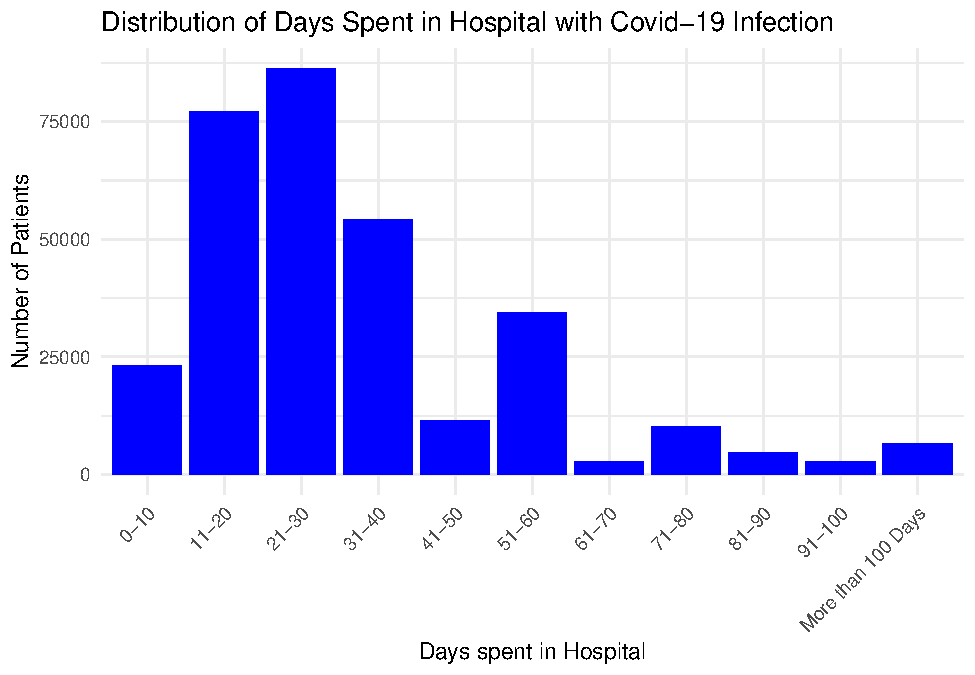
\includegraphics[width=0.9\linewidth]{B273025_final_big_data_rmd_final_files/figure-latex/unnamed-chunk-5-1} 

}

\caption{Distrubution of Days Spent in Hospital due to Covid-19 infection}\label{fig:unnamed-chunk-5}
\end{figure}

Figure 1 shows the distribution of Stay\_Days (LOS). Most patients
stayed 11--30 days, with the highest frequency in the 21--30 day range.
The distribution is right-skewed, highlighting an imbalance in the data,
with stays beyond 40 days being under-represented. This limits the
model's ability to accurately predict these categories accurately.

To address this, stays over 40 days were combined into a single ``above
40 days'' category, improving accuracy from 27.4\% to 33.2\%. However,
category imbalance likely still impacts performance, as discussed in
section 4.

\begin{Shaded}
\begin{Highlighting}[]
\CommentTok{\# Explore relationships between features}
\CommentTok{\# most important feature in model\_v1 was Patient\_Visitors}
\CommentTok{\# Compute boxplot statistics for Patient\_Visitors by Stay\_Days in Spark}
\NormalTok{ldf\_visitors\_boxplot\_stats }\OtherTok{\textless{}{-}}\NormalTok{ sdf\_covid\_hosp }\SpecialCharTok{\%\textgreater{}\%}
  \FunctionTok{group\_by}\NormalTok{(Stay\_Days) }\SpecialCharTok{\%\textgreater{}\%}
  \FunctionTok{summarise}\NormalTok{(}
    \AttributeTok{q1 =} \FunctionTok{percentile\_approx}\NormalTok{(Patient\_Visitors, }\FloatTok{0.25}\NormalTok{), }\CommentTok{\# calculate approximate percentiles on spark dataframe  }
    \AttributeTok{median =} \FunctionTok{percentile\_approx}\NormalTok{(Patient\_Visitors, }\FloatTok{0.5}\NormalTok{),}
    \AttributeTok{q3 =} \FunctionTok{percentile\_approx}\NormalTok{(Patient\_Visitors, }\FloatTok{0.75}\NormalTok{),}
    \AttributeTok{min =} \FunctionTok{min}\NormalTok{(Patient\_Visitors),}
    \AttributeTok{max =} \FunctionTok{max}\NormalTok{(Patient\_Visitors)}
\NormalTok{  ) }\SpecialCharTok{\%\textgreater{}\%}
  \FunctionTok{collect}\NormalTok{() }\CommentTok{\# collect to R dataframe }

\CommentTok{\# Visualise the boxplot using pre{-}computed stats}
\NormalTok{corr\_visitors }\OtherTok{\textless{}{-}} \FunctionTok{ggplot}\NormalTok{(ldf\_visitors\_boxplot\_stats, }\FunctionTok{aes}\NormalTok{(}\AttributeTok{x =} \FunctionTok{as.factor}\NormalTok{(Stay\_Days))) }\SpecialCharTok{+}
  \FunctionTok{geom\_boxplot}\NormalTok{(}
    \FunctionTok{aes}\NormalTok{(}\AttributeTok{ymin =}\NormalTok{ min, }\AttributeTok{lower =}\NormalTok{ q1, }\AttributeTok{middle =}\NormalTok{ median, }\AttributeTok{upper =}\NormalTok{ q3, }\AttributeTok{ymax =}\NormalTok{ max),}
    \AttributeTok{stat =} \StringTok{"identity"}\NormalTok{,}
    \AttributeTok{fill =} \StringTok{"lightblue"}\NormalTok{) }\SpecialCharTok{+}
  \FunctionTok{labs}\NormalTok{(}\AttributeTok{title =} \StringTok{"Number of Visitors by Stay Days"}\NormalTok{,}
       \AttributeTok{x =} \StringTok{"Stay Days"}\NormalTok{,}
       \AttributeTok{y =} \StringTok{"Number of Visitors"}\NormalTok{) }\SpecialCharTok{+}
  \FunctionTok{theme\_minimal}\NormalTok{()}\SpecialCharTok{+}
  \FunctionTok{theme}\NormalTok{(}\AttributeTok{axis.text.x =} \FunctionTok{element\_text}\NormalTok{(}\AttributeTok{angle =} \DecValTok{45}\NormalTok{, }\AttributeTok{hjust =} \DecValTok{1}\NormalTok{)) }\CommentTok{\# Rotate x{-}axis labels}

\NormalTok{corr\_visitors}
\end{Highlighting}
\end{Shaded}

\begin{figure}

{\centering 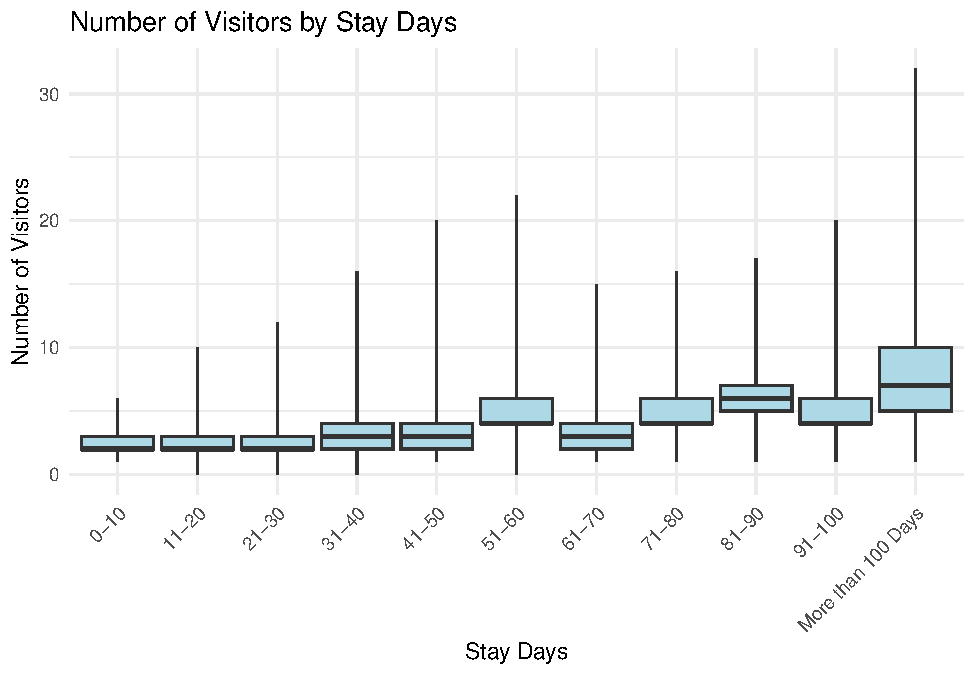
\includegraphics[width=0.9\linewidth]{B273025_final_big_data_rmd_final_files/figure-latex/unnamed-chunk-6-1} 

}

\caption{Figure 2: Relationship between the number of visitors and the length of stay in hospital}\label{fig:unnamed-chunk-6}
\end{figure}

The preliminary model identified Patient\_Visitors as the most important
feature for predicting LOS. Figure 2 shows a positive relationship
between Patient\_Visitors and LOS, indicating it is a dependent variable
and unsuitable for inclusion in the model.

Additionally this feature highlights the importance of designing the
model for real-world use by incorporating only variables known at
admission. Including retrospective variables like Patient\_Visitors
undermines the model's applicability for real-time decision-making.

\section{Fit a Model to the Dataset}\label{fit-a-model-to-the-dataset}

The outcome variable, Stay\_Days, is categorical, requiring a
classification model. Literature suggests Random Forest performs best
for predicting hospital length of stay due to Covid-19 (2,3). This
supervised algorithm uses an ensemble of decision trees created through
bootstrap aggregating (bagging), where subsets of data are sampled with
replacement to train individual trees. Predictions are then averaged
(for regression) or aggregated by majority vote (for classification),
reducing overfitting and improving accuracy.

Random Forest suits this dataset as it handles both numerical and
categorical features without requiring one-hot encoding or extensive
preprocessing. It is robust to high-dimensional data, as it selects
random subsets of features for splitting, making it less prone to
overfitting compared to regression models. Additionally, it provides
feature importance metrics, offering valuable insights into the key
predictors of LOS.

However, Random Forest has limitations, including computational expense
with large datasets and does not inherently provide insights into
feature relationships. Despite these drawbacks, its ability to model
complex, non-linear relationships and handle both categorical and
numerical data efficiently makes it the best choice for this task.

\subsection{Designing a Model}\label{designing-a-model}

I sampled 10\% of the dataset to reduce computational demand and
combined stays over 40 days into a single category, `More than 40,' to
address the imbalance in the right-skewed Stay\_Days distribution. The
dataset was split into 80\% for training and 20\% for testing, with the
training set used to build the model and the test set for evaluation.

\begin{Shaded}
\begin{Highlighting}[]
\CommentTok{\# Sample 10\% of the data (as full dataset takes long time)}
\NormalTok{sdf\_covid\_hosp\_sampled }\OtherTok{\textless{}{-}}\NormalTok{ sdf\_covid\_hosp }\SpecialCharTok{\%\textgreater{}\%}
  \FunctionTok{sdf\_sample}\NormalTok{(}\AttributeTok{fraction =} \FloatTok{0.1}\NormalTok{, }\AttributeTok{replacement =} \ConstantTok{FALSE}\NormalTok{, }\AttributeTok{seed =} \DecValTok{123}\NormalTok{)}

\CommentTok{\# combine stay\_days bucket for above 40 to improve usefulness of the model}
\NormalTok{sdf\_covid\_hosp\_sampled }\OtherTok{\textless{}{-}}\NormalTok{ sdf\_covid\_hosp\_sampled }\SpecialCharTok{\%\textgreater{}\%}
  \FunctionTok{mutate}\NormalTok{(}\AttributeTok{stay\_days\_mutated =} \FunctionTok{case\_when}\NormalTok{(}
\NormalTok{    Stay\_Days }\SpecialCharTok{\%in\%} \FunctionTok{c}\NormalTok{(}\StringTok{"0{-}10"}\NormalTok{, }\StringTok{"11{-}20"}\NormalTok{, }\StringTok{"21{-}30"}\NormalTok{, }\StringTok{"31{-}40"}\NormalTok{) }\SpecialCharTok{\textasciitilde{}}\NormalTok{ Stay\_Days,}
\NormalTok{    Stay\_Days }\SpecialCharTok{\%in\%} \FunctionTok{c}\NormalTok{(}\StringTok{"41{-}50"}\NormalTok{, }\StringTok{"51{-}60"}\NormalTok{, }\StringTok{"61{-}70"}\NormalTok{, }\StringTok{"71{-}80"}\NormalTok{, }\StringTok{"81{-}90"}\NormalTok{, }\StringTok{"91{-}100"}\NormalTok{, }\StringTok{"More than 100 Days"}\NormalTok{) }\SpecialCharTok{\textasciitilde{}} \StringTok{"More than 40"}\NormalTok{))}

\CommentTok{\# Prepare data for model: }
\CommentTok{\# Apply StringIndexer to convert all categorical features into integers for random forest model and remove unnecessary columns:}
\NormalTok{sdf\_covid\_hosp\_stay\_days\_map }\OtherTok{\textless{}{-}}\NormalTok{ sdf\_covid\_hosp\_sampled }\SpecialCharTok{\%\textgreater{}\%}
  \FunctionTok{ft\_string\_indexer}\NormalTok{(}\AttributeTok{input\_col =} \StringTok{"stay\_days\_mutated"}\NormalTok{, }\AttributeTok{output\_col =} \StringTok{"stay\_days\_mutated\_index"}\NormalTok{) }\SpecialCharTok{\%\textgreater{}\%}
  \FunctionTok{ft\_string\_indexer}\NormalTok{(}\AttributeTok{input\_col =} \StringTok{"Department"}\NormalTok{, }\AttributeTok{output\_col =} \StringTok{"Department\_index"}\NormalTok{) }\SpecialCharTok{\%\textgreater{}\%}
  \FunctionTok{ft\_string\_indexer}\NormalTok{(}\AttributeTok{input\_col =} \StringTok{"Ward\_Facility"}\NormalTok{, }\AttributeTok{output\_col =} \StringTok{"Ward\_Facility\_index"}\NormalTok{) }\SpecialCharTok{\%\textgreater{}\%}
  \FunctionTok{ft\_string\_indexer}\NormalTok{(}\AttributeTok{input\_col =} \StringTok{"Ward\_Type"}\NormalTok{, }\AttributeTok{output\_col =} \StringTok{"Ward\_Type\_index"}\NormalTok{) }\SpecialCharTok{\%\textgreater{}\%}
  \FunctionTok{ft\_string\_indexer}\NormalTok{(}\AttributeTok{input\_col =} \StringTok{"Bed\_Grade"}\NormalTok{, }\AttributeTok{output\_col =} \StringTok{"Bed\_Grade\_index"}\NormalTok{) }\SpecialCharTok{\%\textgreater{}\%}
  \FunctionTok{ft\_string\_indexer}\NormalTok{(}\AttributeTok{input\_col =} \StringTok{"Type\_of\_Admission"}\NormalTok{, }\AttributeTok{output\_col =} \StringTok{"Type\_of\_Admission\_index"}\NormalTok{) }\SpecialCharTok{\%\textgreater{}\%}
  \FunctionTok{ft\_string\_indexer}\NormalTok{(}\AttributeTok{input\_col =} \StringTok{"Illness\_Severity"}\NormalTok{, }\AttributeTok{output\_col =} \StringTok{"Illness\_Severity\_index"}\NormalTok{) }\SpecialCharTok{\%\textgreater{}\%} 
  \FunctionTok{ft\_string\_indexer}\NormalTok{(}\AttributeTok{input\_col =} \StringTok{"Age"}\NormalTok{, }\AttributeTok{output\_col =} \StringTok{"Age\_index"}\NormalTok{) }\SpecialCharTok{\%\textgreater{}\%} 
  \FunctionTok{select}\NormalTok{(}\SpecialCharTok{{-}}\NormalTok{patientid, }\SpecialCharTok{{-}}\NormalTok{case\_id, }\SpecialCharTok{{-}}\NormalTok{Stay\_Days, }\SpecialCharTok{{-}}\NormalTok{Department, }\SpecialCharTok{{-}}\NormalTok{Ward\_Facility,}\SpecialCharTok{{-}}\NormalTok{Ward\_Type, }\SpecialCharTok{{-}}\NormalTok{Bed\_Grade, }\SpecialCharTok{{-}}\NormalTok{Type\_of\_Admission, }\SpecialCharTok{{-}}\NormalTok{Illness\_Severity, }\SpecialCharTok{{-}}\NormalTok{Age, }\SpecialCharTok{{-}}\NormalTok{Patient\_Visitors, }\SpecialCharTok{{-}}\NormalTok{Department\_index,}\SpecialCharTok{{-}}\NormalTok{Hospital\_region) }
\CommentTok{\# remove patientid and case\_ID from data set as they are not predictive features}
\CommentTok{\# remove columns with categorical data which have been encoded as integers \_index}
\CommentTok{\# remove Patient\_Visitors as this is a dependent variable, which is not useful in prediction of LOS}
\CommentTok{\# remove features with importance of \textless{}0.01 (Department\_Index, Hospital\_region) to simplify model }
\CommentTok{\# keep in stay\_days\_mutated to enable mapping of index to categories for interpretation of results later in report }

\NormalTok{sdf\_covid\_hosp\_model }\OtherTok{\textless{}{-}}\NormalTok{ sdf\_covid\_hosp\_stay\_days\_map }\SpecialCharTok{\%\textgreater{}\%} 
  \FunctionTok{select}\NormalTok{(}\SpecialCharTok{{-}}\NormalTok{stay\_days\_mutated) }\CommentTok{\# remove stay\_days\_mutated for model, as it is already encoded in stay\_days\_mutated\_index}

\CommentTok{\# \# Persist transformed data to reduce memory and computation costs}
\CommentTok{\# sdf\_covid\_hosp\_model \textless{}{-} sdf\_covid\_hosp\_model \%\textgreater{}\%}
\CommentTok{\#   sdf\_persist(storage.level = "MEMORY\_AND\_DISK")}

\CommentTok{\# Split into training and test sets for evaluation }
\NormalTok{data\_splits }\OtherTok{\textless{}{-}}\NormalTok{ sdf\_covid\_hosp\_model }\SpecialCharTok{\%\textgreater{}\%}
  \FunctionTok{sdf\_random\_split}\NormalTok{(}\AttributeTok{training =} \FloatTok{0.8}\NormalTok{, }\AttributeTok{testing =} \FloatTok{0.2}\NormalTok{, }\AttributeTok{seed =} \DecValTok{123}\NormalTok{)}

\NormalTok{train\_data }\OtherTok{\textless{}{-}}\NormalTok{ data\_splits}\SpecialCharTok{$}\NormalTok{training}
\NormalTok{test\_data }\OtherTok{\textless{}{-}}\NormalTok{ data\_splits}\SpecialCharTok{$}\NormalTok{testing}


\CommentTok{\# Train a Random Forest classifier}
\NormalTok{rf\_model }\OtherTok{\textless{}{-}}\NormalTok{ train\_data }\SpecialCharTok{\%\textgreater{}\%} 
  \FunctionTok{ml\_random\_forest}\NormalTok{(stay\_days\_mutated\_index }\SpecialCharTok{\textasciitilde{}}\NormalTok{.,}\AttributeTok{type =} \StringTok{"classification"}\NormalTok{, }\CommentTok{\# categorical outcome }
                   \AttributeTok{num\_trees =} \DecValTok{100}\NormalTok{, }\CommentTok{\# balance performance and computational cost}
                   \AttributeTok{max\_depth =} \DecValTok{10}\NormalTok{,}
                   \AttributeTok{min\_instances\_per\_node =} \DecValTok{5}\NormalTok{)}

\CommentTok{\# use ml\_predict() to create a Spark data frame that contains the predictions from the testing data set}
\NormalTok{pred }\OtherTok{\textless{}{-}}  \FunctionTok{ml\_predict}\NormalTok{(rf\_model, test\_data)}
\end{Highlighting}
\end{Shaded}

\subsection{Hyperparametric Tuning}\label{hyperparametric-tuning}

Hyperparameter tuning tests combinations of parameters (e.g.,
num\_trees, max\_depth, min\_instances\_per\_node) to find the optimal
model configuration. Below is an example, evaluating 27 combinations of
hyperparameters.

\begin{Shaded}
\begin{Highlighting}[]
\CommentTok{\# \# Not inlcuded code as computer and noteable did not have the storage to execute. }

\CommentTok{\# \# Define the pipeline for Random Forest}
\CommentTok{\# pipeline \textless{}{-} sc \%\textgreater{}\%}
\CommentTok{\#   ml\_pipeline() \%\textgreater{}\%}
\CommentTok{\#   ft\_r\_formula(stay\_days\_mutated\_index \textasciitilde{} .) \%\textgreater{}\% \# Converts data into a formula{-}like structure}
\CommentTok{\#   ml\_random\_forest\_classifier()}
\CommentTok{\# }
\CommentTok{\# \# Define the grid of hyperparameters to test}
\CommentTok{\# grid \textless{}{-} list(random\_forest\_classifier = list(}
\CommentTok{\#     num\_trees = c(50, 100, 150),          \# Test 3 values for number of trees}
\CommentTok{\#     max\_depth = c(5, 10, 15),            \# Test 3 values for maximum tree depth}
\CommentTok{\#     min\_instances\_per\_node = c(1, 5, 10))) \# Test 3 values for minimum instances per node}
\CommentTok{\# }
\CommentTok{\# \# Define the evaluator (accuracy metric for classification)}
\CommentTok{\# evaluator \textless{}{-} ml\_multiclass\_classification\_evaluator(sc, metric\_name = "accuracy") \# measures accuracy of each model during cross{-}validation }
\CommentTok{\# }
\CommentTok{\# \# Set up cross{-}validation}
\CommentTok{\# cv \textless{}{-} ml\_cross\_validator(x = sc,}
\CommentTok{\#   estimator = pipeline,}
\CommentTok{\#   estimator\_param\_maps = grid,}
\CommentTok{\#   evaluator = evaluator,}
\CommentTok{\#   num\_folds = 5,    \# 5{-}fold cross{-}validation}
\CommentTok{\#   parallelism = 4)   \# Use 4 threads for parallel execution}
\CommentTok{\# }
\CommentTok{\# \# Fit the cross{-}validation model}
\CommentTok{\# cv\_model \textless{}{-} ml\_fit(x = cv, dataset = train\_data)}
\CommentTok{\# }
\CommentTok{\# \# Extract validation metrics}
\CommentTok{\# validation\_metrics \textless{}{-} ml\_validation\_metrics(cv\_model)}
\CommentTok{\# }
\CommentTok{\# \# Display validation metrics}
\CommentTok{\# print(validation\_metrics)}
\CommentTok{\# }
\CommentTok{\# \# Select the best model from cross{-}validation}
\CommentTok{\# best\_model \textless{}{-} ml\_best\_model(cv\_model)}
\CommentTok{\# }
\CommentTok{\# \# Evaluate the best model on the test dataset}
\CommentTok{\# test\_predictions \textless{}{-} ml\_predict(best\_model, test\_data)}
\CommentTok{\# test\_metrics \textless{}{-} ml\_evaluate(best\_model, test\_data)}
\CommentTok{\# }
\CommentTok{\# \# Display test metrics}
\CommentTok{\# print(test\_metrics)}
\end{Highlighting}
\end{Shaded}

\section{Evaluation of the Model}\label{evaluation-of-the-model}

\subsection{Main Findings}\label{main-findings}

\begin{Shaded}
\begin{Highlighting}[]
\CommentTok{\# extract importance of each feature and remove features with importance \textless{}0.01 from model}

\NormalTok{ldf\_importance }\OtherTok{\textless{}{-}} \FunctionTok{ml\_feature\_importances}\NormalTok{(rf\_model)  }\CommentTok{\# ldf\_ = local dataframe}

\NormalTok{ldf\_importance }\OtherTok{\textless{}{-}}\NormalTok{ ldf\_importance }\SpecialCharTok{\%\textgreater{}\%} 
  \FunctionTok{ggplot}\NormalTok{(}\FunctionTok{aes}\NormalTok{(}\AttributeTok{x =} \FunctionTok{reorder}\NormalTok{(feature, importance), }\AttributeTok{y =}\NormalTok{ importance)) }\SpecialCharTok{+}
  \FunctionTok{geom\_bar}\NormalTok{(}\AttributeTok{stat =} \StringTok{"identity"}\NormalTok{, }\AttributeTok{fill =} \StringTok{"blue"}\NormalTok{) }\SpecialCharTok{+}
  \FunctionTok{coord\_flip}\NormalTok{() }\SpecialCharTok{+}
  \FunctionTok{labs}\NormalTok{(}\AttributeTok{title =} \StringTok{"Feature Importance"}\NormalTok{, }\AttributeTok{x =} \StringTok{"Feature"}\NormalTok{, }\AttributeTok{y =} \StringTok{"Importance"}\NormalTok{)}\SpecialCharTok{+}
  \FunctionTok{theme\_minimal}\NormalTok{()}

\NormalTok{ldf\_importance}
\end{Highlighting}
\end{Shaded}

\begin{figure}

{\centering 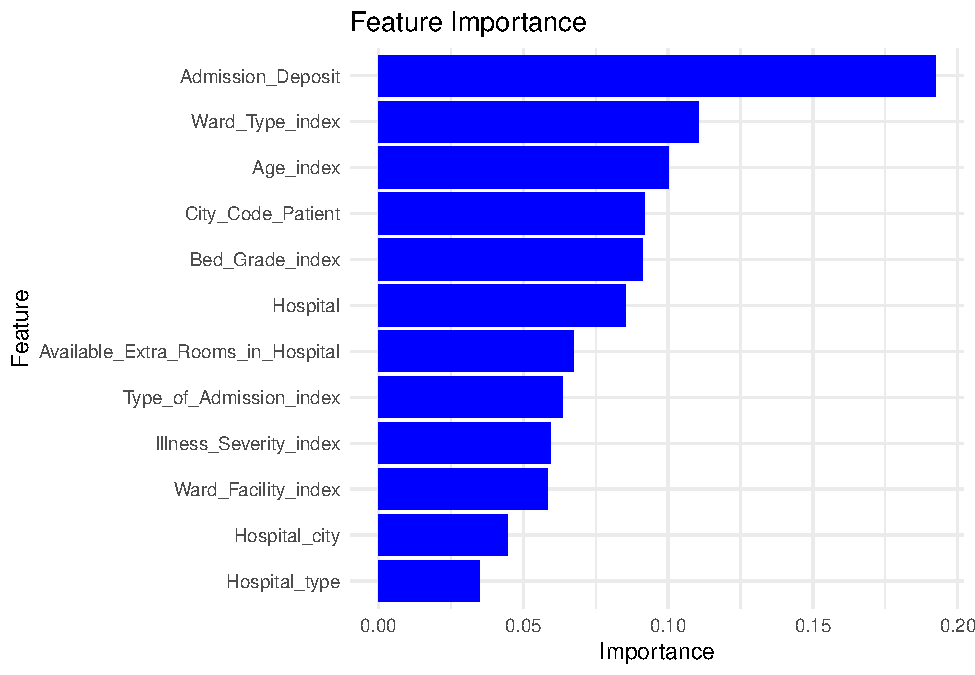
\includegraphics[width=0.9\linewidth]{B273025_final_big_data_rmd_final_files/figure-latex/unnamed-chunk-9-1} 

}

\caption{Ranked Importance of each Feature}\label{fig:unnamed-chunk-9}
\end{figure}

Admission Deposit, Ward Type, Age, and City Code Patient were the most
influential predictors of LOS. Hospital Department and Hospital Region
(\textless0.01\% importance) were excluded from the final model for
simplicity and efficiency.

\subsubsection{Model Performance
Metrics:}\label{model-performance-metrics}

\begin{enumerate}
\def\labelenumi{\arabic{enumi}.}
\tightlist
\item
  Classification Model Metrics
\end{enumerate}

\begin{Shaded}
\begin{Highlighting}[]
\CommentTok{\# Define function to calculate metrics for prediction dataset }
\NormalTok{calculate\_metric }\OtherTok{\textless{}{-}} \ControlFlowTok{function}\NormalTok{(metric\_name) }
\NormalTok{  \{pred }\SpecialCharTok{\%\textgreater{}\%}
    \FunctionTok{ml\_multiclass\_classification\_evaluator}\NormalTok{(}
      \AttributeTok{label\_col =} \StringTok{"label"}\NormalTok{,}
      \AttributeTok{prediction\_col =} \StringTok{"prediction"}\NormalTok{,}
      \AttributeTok{metric\_name =}\NormalTok{ metric\_name)\}}

\CommentTok{\# Create a dataframe and calculate metrics}
\NormalTok{metrics\_df }\OtherTok{\textless{}{-}} \FunctionTok{data.frame}\NormalTok{(}
  \AttributeTok{Metric =} \FunctionTok{c}\NormalTok{(}\StringTok{"Accuracy"}\NormalTok{, }\StringTok{"Precision"}\NormalTok{, }\StringTok{"Recall"}\NormalTok{, }\StringTok{"F1{-}Score"}\NormalTok{),}
  \AttributeTok{Value =} \FunctionTok{c}\NormalTok{(}
    \FunctionTok{calculate\_metric}\NormalTok{(}\StringTok{"accuracy"}\NormalTok{),}
    \FunctionTok{calculate\_metric}\NormalTok{(}\StringTok{"weightedPrecision"}\NormalTok{),}
    \FunctionTok{calculate\_metric}\NormalTok{(}\StringTok{"weightedRecall"}\NormalTok{),}
    \FunctionTok{calculate\_metric}\NormalTok{(}\StringTok{"f1"}\NormalTok{)))}

\CommentTok{\# Make table with gt}
\NormalTok{metrics\_table }\OtherTok{\textless{}{-}}\NormalTok{ metrics\_df }\SpecialCharTok{\%\textgreater{}\%}
  \FunctionTok{gt}\NormalTok{() }\SpecialCharTok{\%\textgreater{}\%}
  \FunctionTok{tab\_header}\NormalTok{(}\AttributeTok{title =} \StringTok{"Model Evaluation Metrics"}\NormalTok{,}
             \AttributeTok{subtitle=}\StringTok{""}\NormalTok{) }\SpecialCharTok{\%\textgreater{}\%}
  \FunctionTok{fmt\_percent}\NormalTok{(}\AttributeTok{columns =} \StringTok{"Value"}\NormalTok{, }\AttributeTok{decimals =} \DecValTok{2}\NormalTok{) }\SpecialCharTok{\%\textgreater{}\%} \CommentTok{\# Limit decimals to 2 places for clarity}
  \FunctionTok{tab\_style}\NormalTok{(}\AttributeTok{style =} \FunctionTok{cell\_text}\NormalTok{(}\AttributeTok{weight =} \StringTok{"bold"}\NormalTok{), }\AttributeTok{locations =} \FunctionTok{cells\_column\_labels}\NormalTok{(}\FunctionTok{everything}\NormalTok{())) }\SpecialCharTok{\%\textgreater{}\%} \CommentTok{\# Bold headers}
  \FunctionTok{opt\_stylize}\NormalTok{(}\AttributeTok{style =} \DecValTok{6}\NormalTok{, }\AttributeTok{color =} \StringTok{"blue"}\NormalTok{)}

\NormalTok{metrics\_table}
\end{Highlighting}
\end{Shaded}

\begin{table}[!t]
\caption*{
{\large Model Evaluation Metrics}
} 
\fontsize{12.0pt}{14.4pt}\selectfont
\begin{tabular*}{\linewidth}{@{\extracolsep{\fill}}lr}
\toprule
{\bfseries Metric} & {\bfseries Value} \\ 
\midrule\addlinespace[2.5pt]
Accuracy & 38.11\% \\ 
Precision & 36.77\% \\ 
Recall & 38.11\% \\ 
F1-Score & 33.20\% \\ 
\bottomrule
\end{tabular*}
\end{table}

The model correctly predicts the LOS for 38.11\% of test cases,
indicating low accuracy and reliability. A precision of 36.77\% shows
many false positives, while a recall of 38.11\% indicates the model
misses a large portion of true cases. The F1-Score of 33.20\% reflects
poor balance between precision and recall. These metrics suggests the
model struggles to capture patterns to accurately predict LOS. This may
result from dataset imbalances, insufficient predictive features or
randomness in LOS.

\begin{enumerate}
\def\labelenumi{\arabic{enumi}.}
\setcounter{enumi}{1}
\tightlist
\item
  Confusion Matrix: Highlights true positives, false positives, true
  negatives and false negatives for each class.
\end{enumerate}

\begin{Shaded}
\begin{Highlighting}[]
\CommentTok{\# Retrieve the mapping of indices to categories}
\NormalTok{ldf\_index\_mapping }\OtherTok{\textless{}{-}}\NormalTok{ sdf\_covid\_hosp\_stay\_days\_map }\SpecialCharTok{\%\textgreater{}\%}
  \FunctionTok{select}\NormalTok{(stay\_days\_mutated, stay\_days\_mutated\_index) }\SpecialCharTok{\%\textgreater{}\%}
  \FunctionTok{distinct}\NormalTok{() }\SpecialCharTok{\%\textgreater{}\%}
  \FunctionTok{arrange}\NormalTok{(stay\_days\_mutated\_index) }\SpecialCharTok{\%\textgreater{}\%}
  \FunctionTok{collect}\NormalTok{()}

\CommentTok{\# Rename the columns in the mapping table for clarity}
\NormalTok{ldf\_index\_mapping }\OtherTok{\textless{}{-}}\NormalTok{ ldf\_index\_mapping }\SpecialCharTok{\%\textgreater{}\%}
  \FunctionTok{rename}\NormalTok{(}\AttributeTok{truth\_index =}\NormalTok{ stay\_days\_mutated\_index,}
    \AttributeTok{truth\_category =}\NormalTok{ stay\_days\_mutated)}

\CommentTok{\# Aggregate counts for confusion matrix in Spark}
\NormalTok{ldf\_confusion\_matrix }\OtherTok{\textless{}{-}}\NormalTok{ pred }\SpecialCharTok{\%\textgreater{}\%}
  \FunctionTok{group\_by}\NormalTok{(}\AttributeTok{truth =}\NormalTok{ label, }\AttributeTok{prediction =}\NormalTok{ prediction) }\SpecialCharTok{\%\textgreater{}\%}
  \FunctionTok{summarise}\NormalTok{(}\AttributeTok{count =} \FunctionTok{n}\NormalTok{(), }\AttributeTok{.groups =} \StringTok{"drop"}\NormalTok{) }\SpecialCharTok{\%\textgreater{}\%}  \CommentTok{\# Compute the counts for each actual{-}predicted pair}
  \FunctionTok{collect}\NormalTok{()}

\CommentTok{\# Join for truth (actual labels)}
\NormalTok{ldf\_confusion\_matrix }\OtherTok{\textless{}{-}}\NormalTok{ ldf\_confusion\_matrix }\SpecialCharTok{\%\textgreater{}\%}
  \FunctionTok{left\_join}\NormalTok{(ldf\_index\_mapping, }\AttributeTok{by =} \FunctionTok{c}\NormalTok{(}\StringTok{"truth"} \OtherTok{=} \StringTok{"truth\_index"}\NormalTok{))}

\CommentTok{\# Rename mapping columns again for predictions}
\NormalTok{ldf\_index\_mapping }\OtherTok{\textless{}{-}}\NormalTok{ ldf\_index\_mapping }\SpecialCharTok{\%\textgreater{}\%}
  \FunctionTok{rename}\NormalTok{(}\AttributeTok{prediction\_index =}\NormalTok{ truth\_index, }\AttributeTok{prediction\_category =}\NormalTok{ truth\_category)}

\CommentTok{\# Join for predictions}
\NormalTok{ldf\_confusion\_matrix }\OtherTok{\textless{}{-}}\NormalTok{ ldf\_confusion\_matrix }\SpecialCharTok{\%\textgreater{}\%}
  \FunctionTok{left\_join}\NormalTok{(ldf\_index\_mapping, }\AttributeTok{by =} \FunctionTok{c}\NormalTok{(}\StringTok{"prediction"} \OtherTok{=} \StringTok{"prediction\_index"}\NormalTok{))}

\CommentTok{\# Select only the readable categories and counts}
\NormalTok{ldf\_confusion\_matrix\_readable }\OtherTok{\textless{}{-}}\NormalTok{ ldf\_confusion\_matrix }\SpecialCharTok{\%\textgreater{}\%}
  \FunctionTok{select}\NormalTok{(truth\_category, }
\NormalTok{    prediction\_category, }
\NormalTok{    count)}

\CommentTok{\# Create a heatmap to visualise confusion matrix }
\NormalTok{confusion\_matrix }\OtherTok{\textless{}{-}} \FunctionTok{ggplot}\NormalTok{(ldf\_confusion\_matrix\_readable, }\FunctionTok{aes}\NormalTok{(}\AttributeTok{x =}\NormalTok{ prediction\_category, }\AttributeTok{y =}\NormalTok{ truth\_category, }\AttributeTok{fill =}\NormalTok{ count)) }\SpecialCharTok{+}
  \FunctionTok{geom\_tile}\NormalTok{(}\AttributeTok{color =} \StringTok{"white"}\NormalTok{) }\SpecialCharTok{+}
  \FunctionTok{scale\_fill\_gradient}\NormalTok{(}\AttributeTok{low =} \StringTok{"\#DDEEFF"}\NormalTok{, }\AttributeTok{high =} \StringTok{"blue"}\NormalTok{) }\SpecialCharTok{+}
  \FunctionTok{labs}\NormalTok{(}\AttributeTok{title =} \StringTok{"Confusion Matrix"}\NormalTok{,}
    \AttributeTok{x =} \StringTok{"Predicted Category"}\NormalTok{,}
    \AttributeTok{y =} \StringTok{"Actual Category"}\NormalTok{) }\SpecialCharTok{+}
  \FunctionTok{theme\_minimal}\NormalTok{()}

\NormalTok{confusion\_matrix}
\end{Highlighting}
\end{Shaded}

\begin{figure}

{\centering 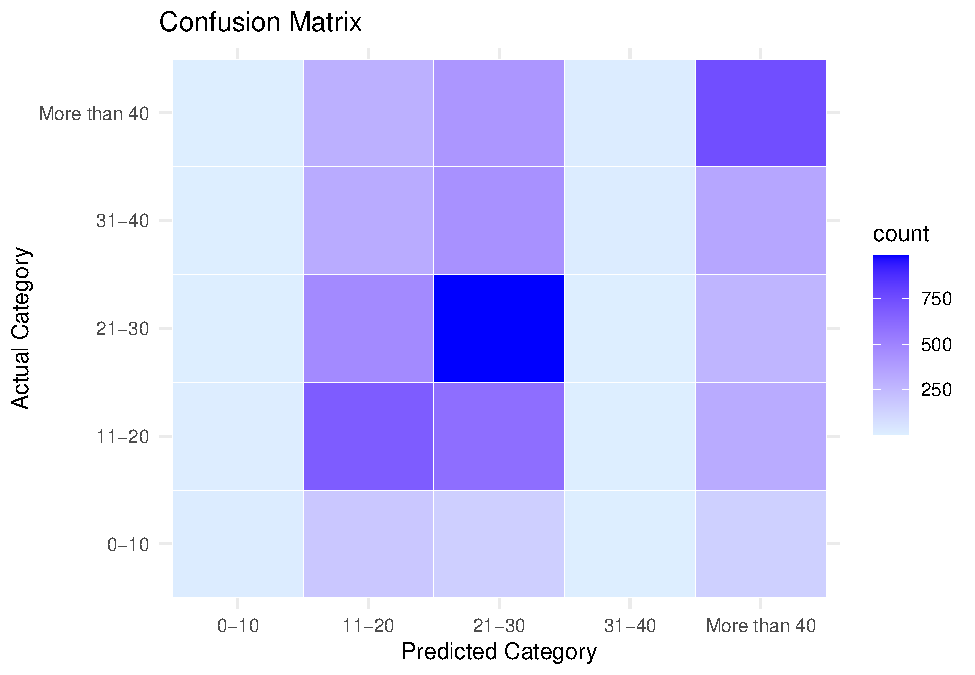
\includegraphics[width=0.9\linewidth]{B273025_final_big_data_rmd_final_files/figure-latex/unnamed-chunk-11-1} 

}

\caption{Confusion Matrix}\label{fig:unnamed-chunk-11}
\end{figure}

The confusion matrix reveals that the model performs best at predicting
the 21-30 and More\_than\_40 categories, which have the most data,
indicating the model is bias towards majority classes. Categories such
as 0-10 and 31-40, with fewer samples (n=31 and n=40), are rarely
predicted correctly. This imbalance limits the model's ability to learn
patterns for under-represented categories, a common issue with Random
Forest models when faced with imbalanced datasets.

\subsection{Strengths and Weaknesses of the
Approach:}\label{strengths-and-weaknesses-of-the-approach}

Strengths:

\begin{enumerate}
\def\labelenumi{\arabic{enumi}.}
\tightlist
\item
  \textbf{Robustness to Overfitting:} Random Forest good choice for
  complex datasets consisting of many features with non-linear
  relationships.
\item
  \textbf{Interpretability:} Importance metrics highlight key predictors
  of LOS which can guide decision-making and further analysis.
\item
  \textbf{Handling of Mixed Data:} The model effectively processes both
  numerical and categorical features without extensive preprocessing.
\end{enumerate}

Weaknesses:

\begin{enumerate}
\def\labelenumi{\arabic{enumi}.}
\tightlist
\item
  \textbf{Poor Predictive Power:} Low accuracy and F1-Score suggest the
  model is not effectively capturing patterns in the data.
\item
  \textbf{Bias Toward Majority Classes:} Under-representation of
  minority categories skews predictions.
\item
  \textbf{Limited Real-World Applicability:} Predictions lack
  reliability for real-world decisions.
\item
  \textbf{Computational Cost:} Training and evaluating Random Forest
  models are resource-intensive for large datasets.
\end{enumerate}

\subsection{Broader Implications of
Analysis}\label{broader-implications-of-analysis}

Future Random Forest models must address class imbalance to improve
predictions for under-represented categories. Techniques such as
oversampling minority classes, under sampling majority classes, or
making the weight of each class a feature in the model can be used to
ensure categories are equally represented.

This dataset may lack critical features which determine LOS limiting
accuracy. Prospective studies such as ISARIC4C CO-CIN gathered more
parameters on admission characteristics and hospital resource
utilisation which allowed development of robust models which informed
public health policy in the UK.(4,5) Additionally, this analysis
highlights the importance of selecting features known at admission for
real-time applicability.

This model's low accuracy and reliability make it unsuitable for
actionable decision-making. A simpler approach, such as setting a
threshold and grouping outcomes (e.g., \textless30 days
vs.~\textgreater30 days), may enhance performance.

Insights from this analysis can guide predictive tools for future
pandemics, aiding healthcare system preparedness.

\section{References}\label{references}

\begin{enumerate}
\def\labelenumi{\arabic{enumi}.}
\item
  Rees EM, Nightingale ES, Jafari Y, Waterlow NR, Clifford S, Pearson
  CA, et al.~COVID-19 length of hospital stay: a systematic review and
  data synthesis. \emph{BMC Medicine} {[}Internet{]}. 2020 Sep 3
  {[}cited 2024 Dec 11{]};18(1):270. Available from:
  \url{https://doi.org/10.1186/s12916-020-01726-3}
\item
  Alabbad DA, Almuhaideb AM, Alsunaidi SJ, Alqudaihi KS, Alamoudi FA,
  Alhobaishi MK, et al.~Machine learning model for predicting the length
  of stay in the intensive care unit for COVID-19 patients in the
  eastern province of Saudi Arabia. \emph{Informatics in Medicine
  Unlocked} {[}Internet{]}. 2022 {[}cited 2024 Dec 11{]};30:100937.
  Available from:
  \url{https://www.ncbi.nlm.nih.gov/pmc/articles/PMC9010025/}
\item
  Samy SS, Karthick S, Ghosal M, Singh S, Sudarsan JS, Nithiyanantham S.
  Adoption of machine learning algorithm for predicting the length of
  stay of patients (construction workers) during COVID pandemic.
  \emph{International Journal of Information Technology} {[}Internet{]}.
  2023 Jun 1 {[}cited 2024 Dec 11{]};15(5):2613--21. Available from:
  \url{https://doi.org/10.1007/s41870-023-01296-6}
\item
  Keogh RH, Diaz-Ordaz K, Jewell NP, Semple MG, de Wreede LC, Putter H,
  et al.~Estimating distribution of length of stay in a multi-state
  model conditional on the pathway, with an application to patients
  hospitalised with Covid-19. \emph{Lifetime Data Anal} {[}Internet{]}.
  2023 Apr 1 {[}cited 2024 Dec 12{]};29(2):288--317. Available from:
  \url{https://doi.org/10.1007/s10985-022-09586-0}
\item
  Leclerc QJ, Fuller NM, Keogh RH, Diaz-Ordaz K, Sekula R, Semple MG, et
  al.~Importance of patient bed pathways and length of stay differences
  in predicting COVID-19 hospital bed occupancy in England. \emph{BMC
  Health Serv Res} {[}Internet{]}. 2021 Jun 9 {[}cited 2024 Dec
  12{]};21(1):566. Available from:
  \url{https://doi.org/10.1186/s12913-021-06509-x}
\end{enumerate}

Word Count = 1044 words (excluding titles, code chunks \& references)
Figures/Tables = 6

\begin{Shaded}
\begin{Highlighting}[]
\FunctionTok{spark\_disconnect\_all}\NormalTok{(sc)}
\end{Highlighting}
\end{Shaded}

\begin{verbatim}
## [1] 1
\end{verbatim}

\end{document}
